\documentclass[a4paper, 12pt]{article}
\usepackage{graphicx}

\renewcommand{\thesubsection}{\thesection.\alph{subsection}}


\usepackage{xparse}
\ExplSyntaxOn
\NewDocumentCommand{\Rowvec}{ O{,} m }
{
	\vector_main:nnnn { p } { & } { #1 } { #2 }
}
\NewDocumentCommand{\Colvec}{ O{,} m }
{
	\vector_main:nnnn { p } { \\ } { #1 } { #2 }
}

\seq_new:N \l__vector_arg_seq
\cs_new_protected:Npn \vector_main:nnnn #1 #2 #3 #4
{
	\seq_set_split:Nnn \l__vector_arg_seq { #3 } { #4 }
	\begin{#1matrix}
		\seq_use:Nnnn \l__vector_arg_seq { #2 } { #2 } { #2 }
	\end{#1matrix}
}
\ExplSyntaxOff

\usepackage{enumitem}
\usepackage{t1enc}
\usepackage[utf8]{inputenc}
\usepackage[magyar]{babel}

% a szép matematikai szimbólumokért
\usepackage{amssymb}
\usepackage{amsmath}
\usepackage{nccmath}
\usepackage{siunitx}

\usepackage{listings}
\lstset{language=Python}

\usepackage{subcaption}
\usepackage[justification=centering]{caption}

% ha táblázatban szeretnénk egyesített sorokat is
\usepackage{multirow}

% horizontal line
\usepackage{hhline}

% eps formátumú ábrák --> pdflatex fordításhoz!!
\usepackage{epsfig}

% egyenletekhez, pl mátrixok írására
\usepackage{array}

% ha betűszíneket is szeretnénk használni
\usepackage{color}

% Margók egyéni beállításai
\usepackage{anysize}
\marginsize{1.64cm}{1.64cm}{1.2cm}{2.4cm} %\left right top bottom

% vakszöveg
\usepackage{lipsum}
\usepackage{blindtext}

% A HIVATKOZÁSOKHOZ HASZNÁLT CSOMAGOK. RÉSZLETESEBBEN LD: google -> latex bibtex
\usepackage[numbers, square, comma, sort&compress]{natbib}
%\usepackage[format=hang,labelsep=period]{caption}

\usepackage[unicode]{hyperref}   % ezzel a hivatkozások linkké válnak
\usepackage{bookmark}
\hypersetup{bookmarksopen={true}}
\hypersetup{bookmarksopenlevel={2}}
\hypersetup{bookmarksnumbered={true}}
\hypersetup{
	colorlinks,%
	citecolor=red,%
	filecolor=black,%                                                                                                                                               
	linkcolor=blue,%
	urlcolor=green
}
\numberwithin{equation}{section}          % ezekkel tudod beállítani, hogy milyen felbontásig menjen a hivatkozás
\numberwithin{figure}{subsection}
%\numberwithin{table}{section}          % ha kikommenteled, akkor csak simán számozva lesz.

%%%%%%%%%%%%%%%% Néhány dolog a fancy kinézethez

\frenchspacing
\setlength{\parskip}{2ex}
\setlength{\headsep}{1cm}
\setlength{\headheight}{4pt}

% fej- es lábléc
\usepackage{fancyhdr}
\usepackage{fancyref}
\usepackage{fancyvrb}
\pagestyle{fancy}

\renewcommand{\headrulewidth}{2pt}
\renewcommand{\footrulewidth}{0pt}


\fancyhf{}
\fancyhead[LO]{{ \nouppercase{\rightmark}} }

\cfoot{--~\thepage~--}

%%%%%%%%%%%%%%%%%%%%%%%%%%%


%%%%%%%%%%%%%%%%%%%%%%%%%%%%%%%%%%%%%%%%%%%%%%%%%%%%%%%%%%%%%%%%%%%%%%%%%%%%

\begin{document}

% Címoldalt lehet egyszerűen a \maketitle paranccsal is. Ha kissé részletesebb
% címre van szükség, azt lehet így is, kézzel megadva mindent.
\begin{titlepage}   
\begin{center}
\thispagestyle{empty}  

\vspace*{0.7cm}
\rule{\linewidth}{0.5mm} \\[3mm]
\vspace*{0.7cm}

{\LARGE Véletlen fizikai folyamatok}

\vspace*{0.7cm}
\rule{\linewidth}{0.5mm} \\[3mm]
\rule{\linewidth}{0.5mm} \\[3mm]



{\Large 8. beadandó\\}

\vspace*{0.7cm}
\rule{\linewidth}{0.5mm} \\[3mm]
  {\small Márton Tamás} \\[3mm]
{\footnotesize PJF19C} \\
{\footnotesize martontamas@caesar.elte.hu}

  \vspace*{2cm}

\begin{figure}[h!]
\begin{center}

\includegraphics[width=0.5\textwidth]{./elte.png}
\end{center}
\end{figure}

\end{center}
\end{titlepage}

\newpage

%%%%%%%%%%%%%%%%%%%%%%%%%%%%%%%%%%%%%%%%%%%%%%%%%%%%%%%%%%%%%%%%%%%%%%%%

\thispagestyle{empty}  

%1
\section{feladat}

\begin{center}
\underline{Feladat leírás.}
\end{center}

\begin{figure}[h!]
	\begin{center}
		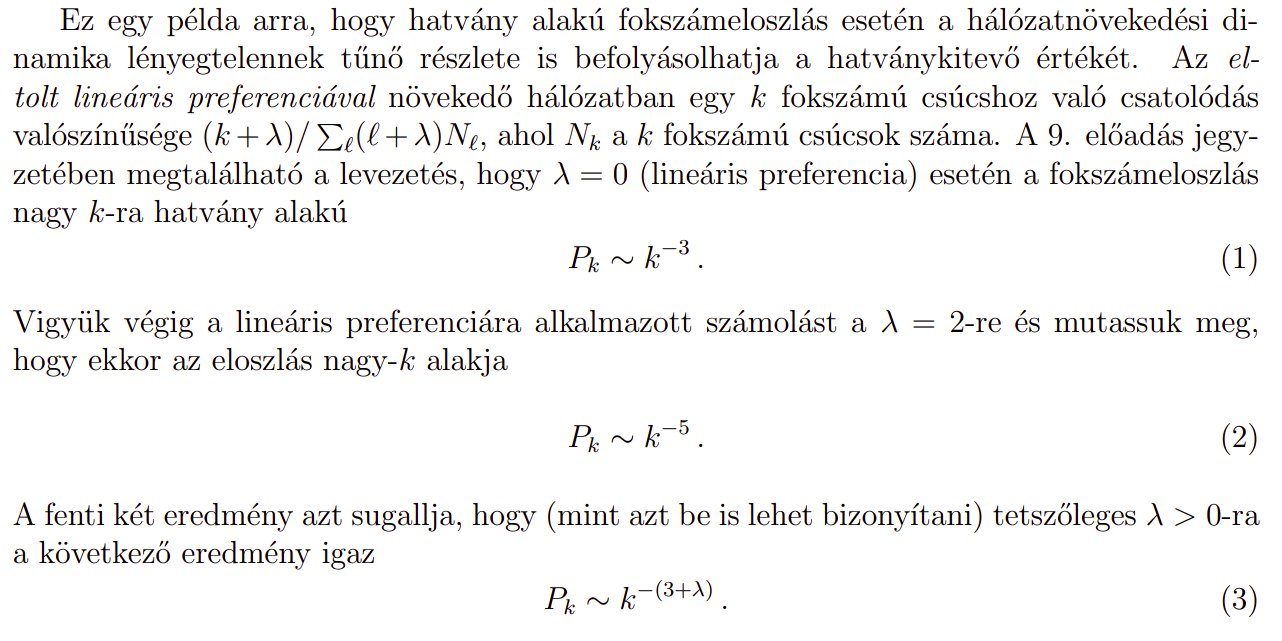
\includegraphics[width=1\textwidth]{elsof.png}
	\end{center}
\end{figure}

\begin{center}
\underline{Feladat megoldása.}
\end{center}
\hspace{5cm}

Az előadási példához hasonlóan, ahol a rátát $w_k = \frac{k}{A}$ alakban írtuk fel, így vizsgáljuk most is \textit{A} értékét:

\begin{center}
	\begin{equation}
	A = \sum_{l = 1}^{N} = (l + \lambda)N_l = 2N + \lambda N = (2 + \lambda)N
	\end{equation}
	\label{A}
\end{center}

Írjuk fel a Master-egyenletet a rendszerünkre:

\begin{center}
\begin{gather*}
N_k(N+1) = N_k(N) - \frac{k + \lambda}{A}N_k + \frac{k+\lambda-1}{A}N_{k-1}\\
N_1(N+1) = N_1(N) - \frac{1 + \lambda}{A}N_1 +1,
\end{gather*}
\end{center}
\clearpage
ami a következő alakra hozható:
\begin{center}
	\begin{gather*}
	\frac{dN_k}{dN} =  - \frac{k + \lambda}{A}N_k + \frac{k+\lambda-1}{A}N_{k-1}\\
	\frac{dN_1}{dN} = - \frac{1 + \lambda}{A}N_1 +1,
	\end{gather*}
\end{center}

valamint behelyettesítem az \textit{A} ra kapott értéket(\ref{A}):

\begin{center}
	\begin{gather*}
	\frac{dN_k}{dN} =  - \frac{k + \lambda}{(2 + \lambda)N}N_k + \frac{k+\lambda-1}{(2 + \lambda)N}N_{k-1}\\
	\frac{dN_1}{dN} = - \frac{1 + \lambda}{(2 + \lambda)N}N_1 +1,
	\end{gather*}
\end{center}

valamint alkalmazom a $\lambda = 2$ helyettesítési értéket:

\begin{center}
	\begin{gather*}
	\frac{dN_k}{dN} =  - \frac{k + 2}{4N}N_k + \frac{k+1}{4N}N_{k-1}\\
	\frac{dN_1}{dN} = - \frac{3}{4N}N_1 +1.
	\end{gather*}
\end{center}

Kihasználom, hogy a fokszámeloszlás definíciója:


\begin{center}
	\begin{equation}
P_k = \frac{N_k}{N}.
	\end{equation}
\end{center}


Ekkor az egyenlet az alábbi alakra hozható:
\begin{center}
	\begin{gather*}
	\frac{dN_k}{dN} =  - \frac{k + 2}{4}P_k + \frac{k+1}{4}P_{k-1}\\
	\frac{dN_1}{dN} = - \frac{3}{4}P_1 +1.
	\end{gather*}
\end{center}

Valamint tudjuk, hogy:

\begin{center}
	\begin{equation}
	\frac{dN_k}{dN} = \frac{d(NP_k)}{dN} = P_k + N\frac{dP_k}{dN},
	\end{equation}
\end{center}

ezért át tudom írni a Master-egyenletemet a fokszámeloszlásra vonatkozó differenciálegyenletekké:

\begin{center}
	\begin{gather*}
	P_k+N\frac{dP_k}{dN} =  - \frac{k + 2}{4}P_k + \frac{k+1}{4}P_{k-1}\\
	P_1 +N\frac{dP_1}{dN} = - \frac{3}{4}P_1 +1.
	\end{gather*}
\end{center}

Majd átrendezem az egyenletet:

\begin{center}
	\begin{gather*}
	N\frac{dP_k}{dN} =  - \frac{k + 6}{4}P_k + \frac{k+1}{4}P_{k-1}\\
	N\frac{dP_1}{dN} = - \frac{7}{4}P_1 +1.
	\end{gather*}
\end{center}

Tudjuk, hogy stacionárius megoldásnál az összes derivált zérus, így:
\begin{center}
	\begin{gather*}
	P_k^{stac} =  - \frac{k}{k+5}P_{k-1}^{stac} = \frac{k(k-1)}{(k+5)(k+4)}P_{k-2}^{stac} =... = \frac{k!}{(k+5)!}P_1^{stac}\\
	P_1^{stac} = \frac{4}{7}.
	\end{gather*}
\end{center}

Ha megvizsgálom külön a $P_k$ fokszámeloszlását, akkor:

\begin{center}
	\begin{gather*}
	P_k^{stac} = \frac{k!}{(k+5)!}\cdot \frac{4}{7} = \frac{4}{7} \cdot \frac{1}{(k+5)(k+4)(k+3)(k+2)(k+1)} \approx \frac{1}{k^5}.
	\end{gather*}
\end{center}
Tehát megkaptuk a helyes végeredményt, miszerint $P_k \approx k^{-(3+\lambda)}$, azaz ha $\lambda = 2$ akkor $P_k \approx k^{-5}$
\clearpage
%2
\section{feladat}

\begin{center}
	\underline{Feladat leírás.}
\end{center}

\begin{figure}[h!]%
	\begin{center}
		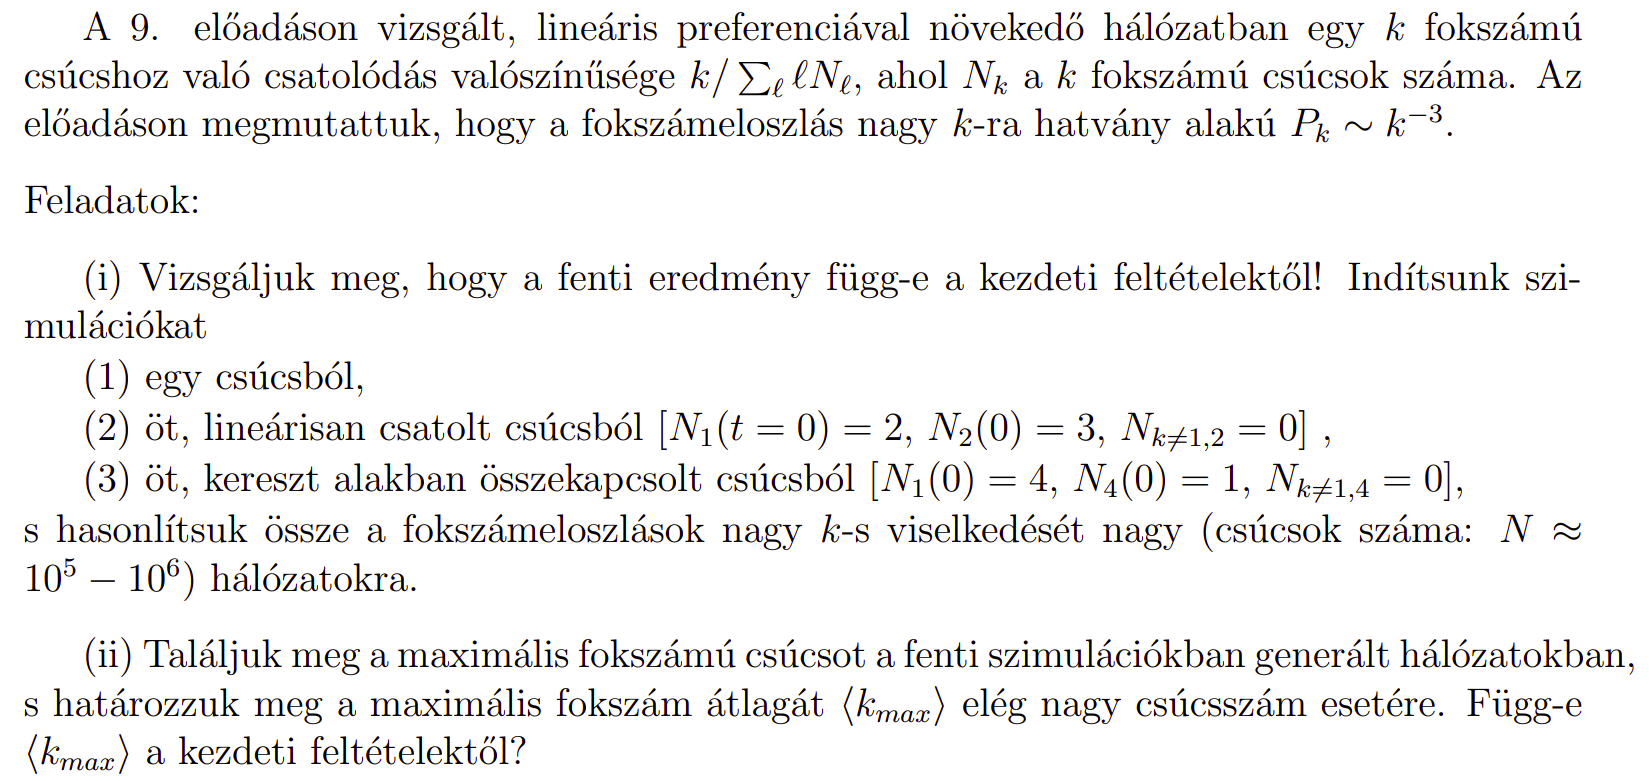
\includegraphics[width=1\textwidth]{masodikf.png}
	\end{center}
\end{figure}

\begin{center}
	\underline{Feladat megoldása.}
\end{center}

A hálózat szimulációját \textit{Pythonban} írtam \textit{Jupyter-notebook}-ban.\\
Az \textit{(1),(2),(3)} feladat megoldásához létrehoztam a fokszámokat: 
\newline
\rule{\textwidth}{0.1pt}
\begin{lstlisting}
############ (1) feladathoz 
fokszamok[0] = 1
fokszamok[1] = 1
melyikhez_keruljon_a_harmas = randint(0,2)
fokszamok[2] = 1
fokszamok[melyikhez_keruljon_a_harmas] += 1
############ (2) feladathoz 
fokszamok[0] = 2
fokszamok[1] = 2
fokszamok[2] = 2
fokszamok[3] = 1
fokszamok[4] = 1
\end{lstlisting}
\rule{\textwidth}{0.1pt}


\clearpage
\begin{lstlisting}
############ (3) feladathoz 
fokszamok[0] = 4
fokszamok[1] = 1
fokszamok[2] = 1
fokszamok[3] = 1
fokszamok[4] = 1
\end{lstlisting}
\rule{\textwidth}{0.1pt}

A szimulációhoz, az adatok kiszámolásához egy törzset használtam, különböző $N$ értékek mellett.
A szimuláció lépései a következők voltak:
\begin{itemize}
	\item kiválasztunk egy mar lent levő csúcsot véletlenszerűen,
	\item leszámoljuk a kivalásztott csúcs éleinek számát \textit{fokszám=k},
	\item kiválasztott csúcshoz $w_k$ valószínűséggel kötöm az új berakott csúcsot,
	\item $w_k = k/A$,
	\item $A = \sum l*Nl$ ahol $Nl$ az l éllel rendelkező csúcsok száma,
	\item húzok egy számot véletlenszerűen $[0,1]$ között,
	\item ha a random szám $< w_k$, hozzákötöm a csúcshoz, ha nem, választok új csúcsot es előröl kezdem a folyamatot,
	\item a (2) és a (2) feladat eseteben a szimuláció \textit{for} ciklusa \textit{(5,N)} között fut.	
\end{itemize}

\rule{\textwidth}{0.1pt}
\begin{lstlisting}
for i in range (3,N):
	osszekotes_megtortent = False
	A = 0
	A_szamolva_volt_e = False

	while (osszekotes_megtortent == False):
		random_kivalasztott_csucs = randint(0,i)
		k = fokszamok[random_kivalasztott_csucs]

	if(A_szamolva_volt_e == False):
		for j in range (0,i):
		A += fokszamok[j]
		A_szamolva_volt_e = True
\end{lstlisting}
\rule{\textwidth}{0.1pt}
\clearpage
\rule{\textwidth}{0.1pt}
\begin{lstlisting}
	w_k = k / A
	P = random.random()

	if(P < w_k):
		fokszamok[random_kivalasztott_csucs] += 1
		fokszamok[i] = 1
		osszekotes_megtortent = True
\end{lstlisting}
\rule{\textwidth}{0.1pt}

Majd a legnagyobb fokszámmal rendelkező csúcsot kerestem meg és ennek kiírását oldottam meg, valamint az ábrázoláshoz készítettem elő az adatokat, ami az analitikus görbét is tartalmazza.
\newline
\rule{\textwidth}{0.1pt}
\begin{lstlisting}
#Legnagyobb fokszamu csucs megtalalasa
index = where(fokszamok == max(fokszamok))
print("Az ennyiedik csucs(ok)nak van maximalis fokszama: " +
	str(csucsok[index[0]]) + " ami ekkora fokszamu: " + 
	str(max(fokszamok)))

#unique-izalas
fokszameloszlas = []
fokszamokfajtaja = []
for i in range (0,N):
	if fokszamok[i] not in fokszamokfajtaja:
		fokszamokfajtaja.append(fokszamok[i])
		fokszameloszlas.append(1)
	if fokszamok[i] in fokszamokfajtaja:
		fokszameloszlas[fokszamokfajtaja.index(fokszamok[i])] += 1

#kiiratas
for i in range (0,len(fokszameloszlas)):
	print("Mekkora fokszam: " + str(fokszamokfajtaja[i]) + 
	". Ennek gyakorisaga:"+str(fokszameloszlas[i]))

fokszameloszlas = numpy.array(fokszameloszlas)
fokszamokfajtaja = numpy.array(fokszamokfajtaja)
eloszlasfuggveny = fokszameloszlas / N

#analitikus mo
def analitikus_mo(k):
	return 1/(k**3)

k = linspace(1,max(fokszamokfajtaja),1000)

\end{lstlisting}
\rule{\textwidth}{0.1pt}


\clearpage

Ábrázoltam a szimuláció eredményeit, melyen látható, hogy a három különböző kezdőparaméterekkel rendelkező rendszerek, mennyire térnek el a $P_k \approx k^{-3}$ alaktól.
Az ábrákról leolvasható, hogy kellően nagy $N$-ekre a rendszer  megközelíti az elméleti értéket  a logaritmikus skálás ábrázolt értékeken jól látszik hogy növekvő $N$-ek esetén, hogyan mozognak a szimulált adatok, sajnos számítási kapacitás hiányában nem tudtam a $10^5-10^6$-os tartományig elmenni, mivel a számítógépem nem engedte, de az $N=100$ as feltétel mellett jól megfigyelhető az eltérés.

\textbf{1.részfeladat}\newline


\begin{figure}[h!]
	\begin{center}
		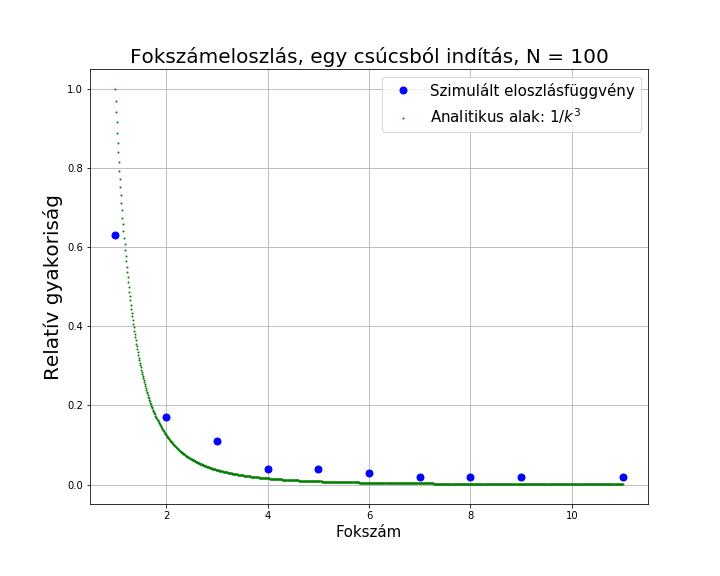
\includegraphics[width=1\textwidth]{elso100.png}
	\end{center}
\end{figure}
\clearpage

\begin{figure}[c]
	\begin{center}
		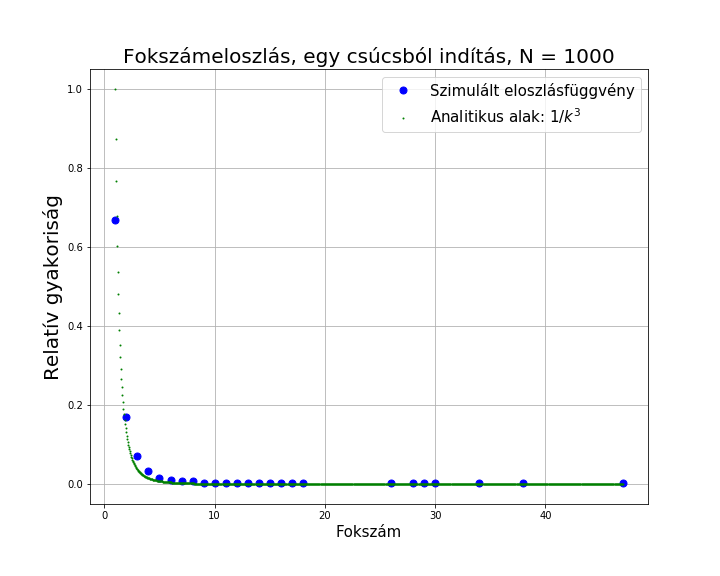
\includegraphics[width=1\textwidth]{elso1000.png}
	\end{center}
\end{figure}

\begin{figure}[c!]
	\begin{center}
		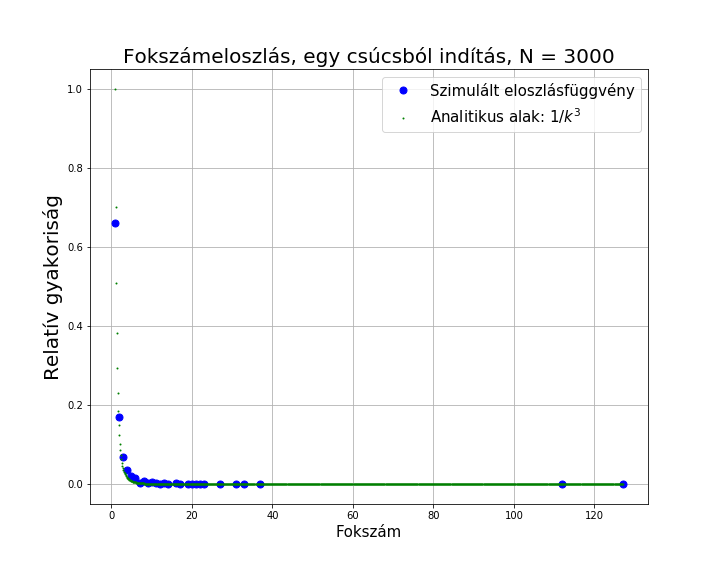
\includegraphics[width=1\textwidth]{elso.png}
	\end{center}
\end{figure}



\clearpage

\begin{figure}[h!]
	\begin{center}
		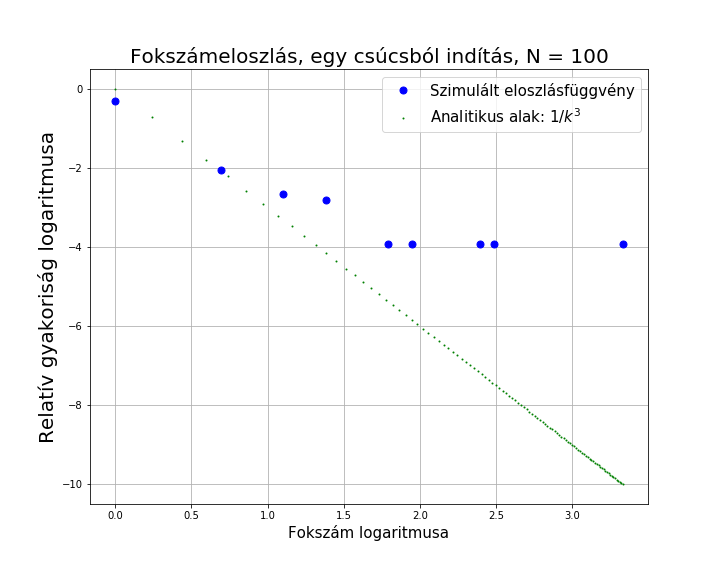
\includegraphics[width=1\textwidth]{elsolog.png}
	\end{center}
\end{figure}
\clearpage

\begin{figure}[c]
	\begin{center}
		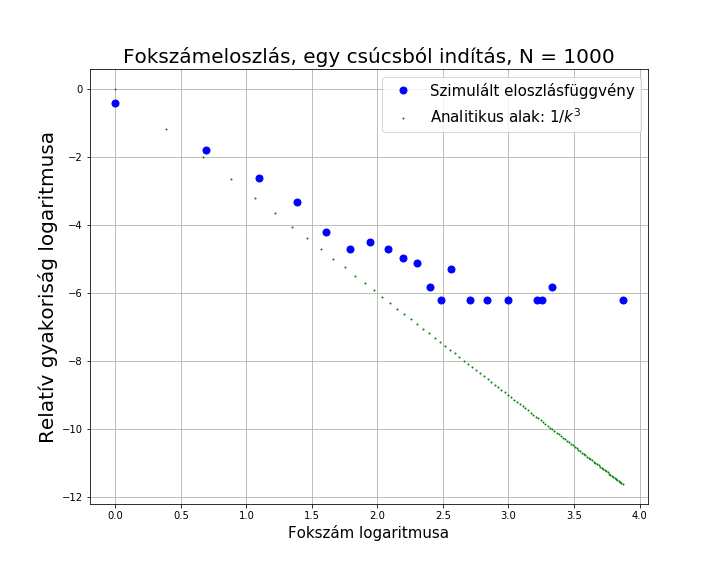
\includegraphics[width=1\textwidth]{elso1000log.png}
	\end{center}
\end{figure}

\begin{figure}[c!]
	\begin{center}
		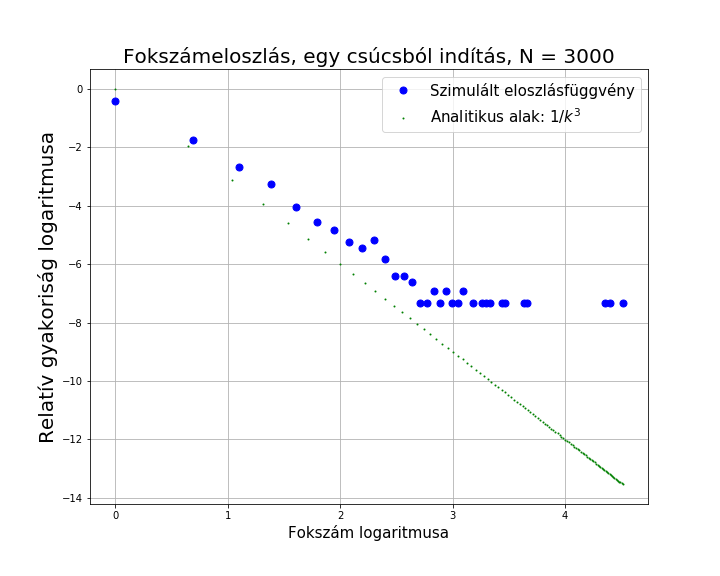
\includegraphics[width=1\textwidth]{elso3000log.png}
	\end{center}
\end{figure}



\clearpage

\textbf{2.részfeladat}\newline

\begin{figure}[ch!]
	\begin{center}
		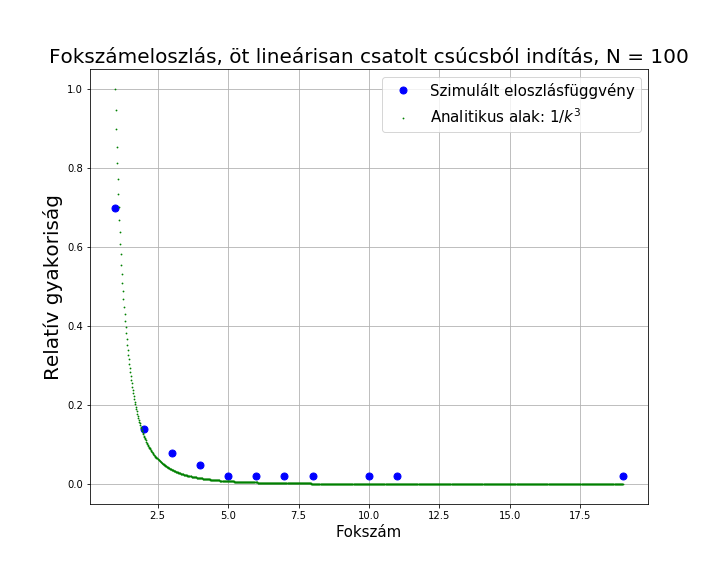
\includegraphics[width=1\textwidth]{masodik100.png}
	\end{center}
\end{figure}
\clearpage
\begin{figure}[c!]
	\begin{center}
		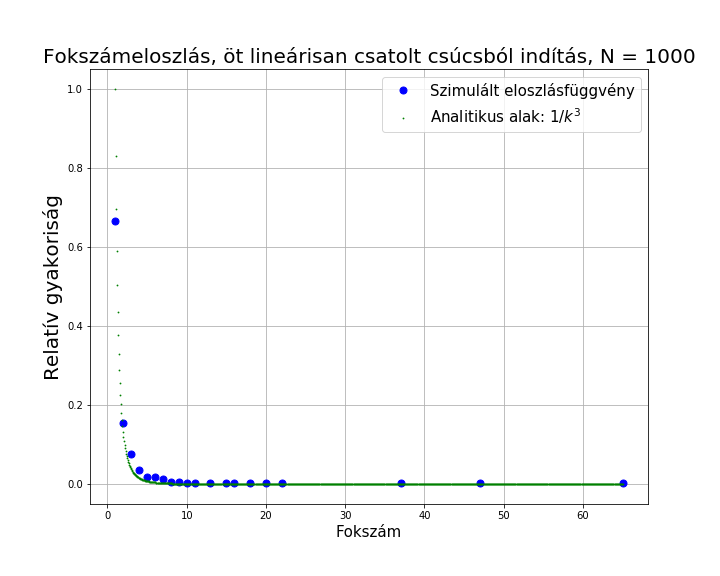
\includegraphics[width=1\textwidth]{masodik1000.png}
	\end{center}
\end{figure}
\clearpage
\begin{figure}[c!]
	\begin{center}
		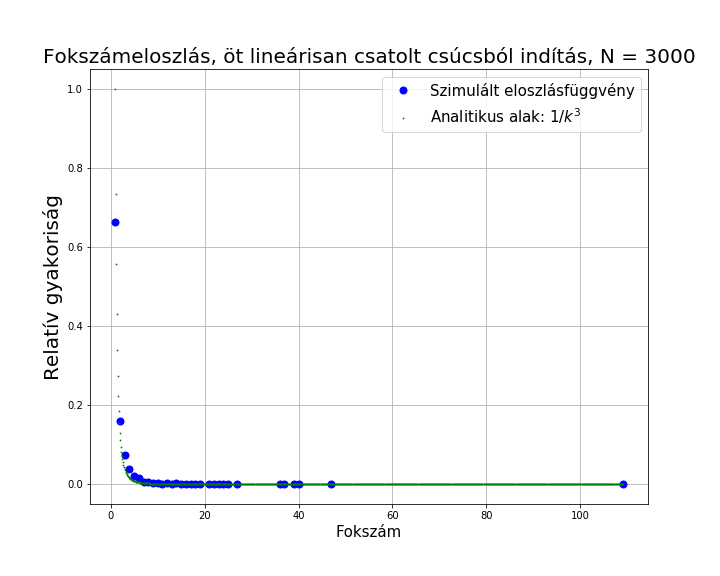
\includegraphics[width=1\textwidth]{masodik.png}
	\end{center}
\end{figure}

\clearpage

\begin{figure}[ch!]
	\begin{center}
		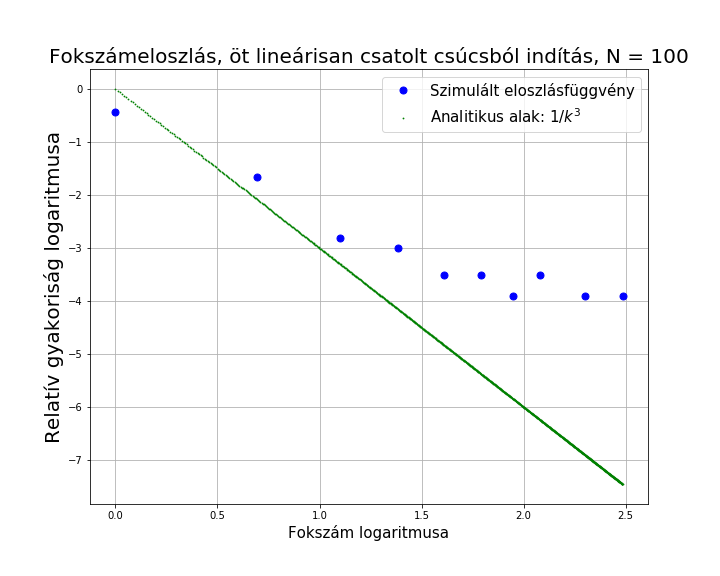
\includegraphics[width=1\textwidth]{masodik100log.png}
	\end{center}
\end{figure}
\clearpage
\begin{figure}[c!]
	\begin{center}
		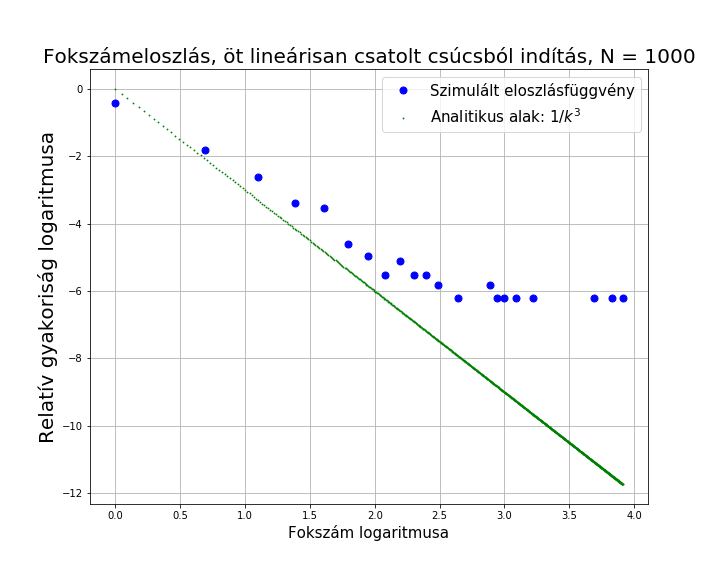
\includegraphics[width=1\textwidth]{masodik1000log.png}
	\end{center}
\end{figure}
\clearpage
\begin{figure}[c!]
	\begin{center}
		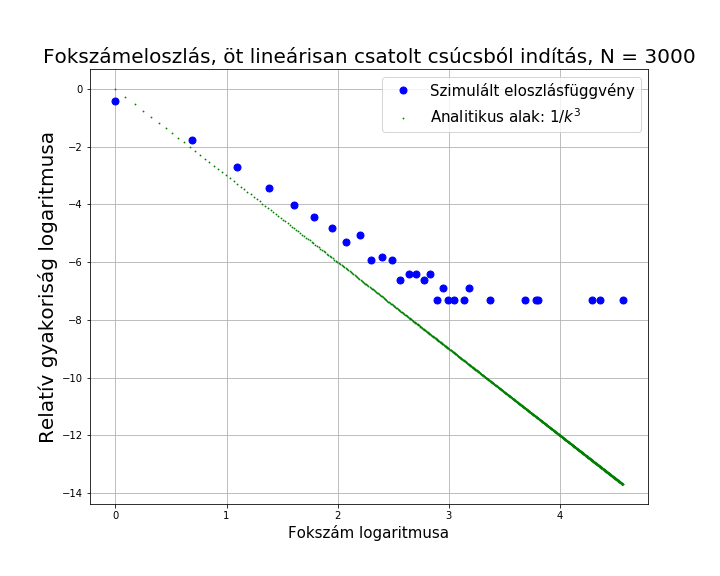
\includegraphics[width=1\textwidth]{masodik3000log.png}
	\end{center}
\end{figure}

\clearpage


\textbf{3.részfeladat}\newline


\begin{figure}[ch!]
	\begin{center}
		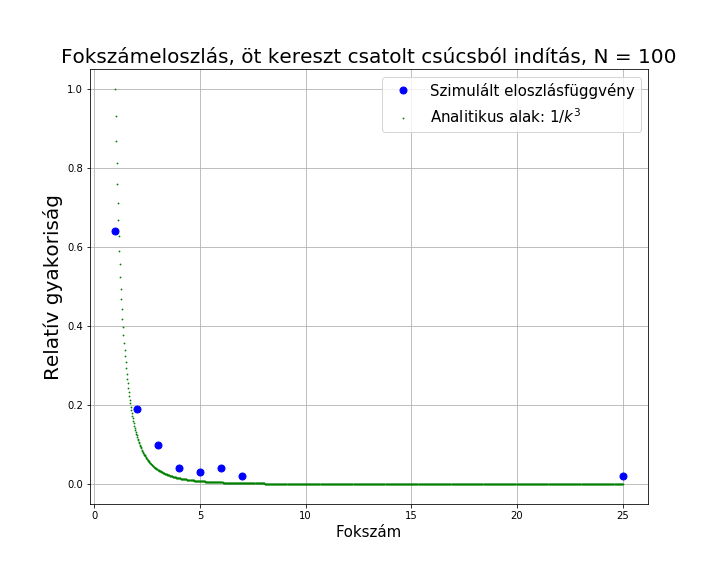
\includegraphics[width=1\textwidth]{harmadik100.png}
	\end{center}
\end{figure}
\clearpage
\begin{figure}[c!]
	\begin{center}
		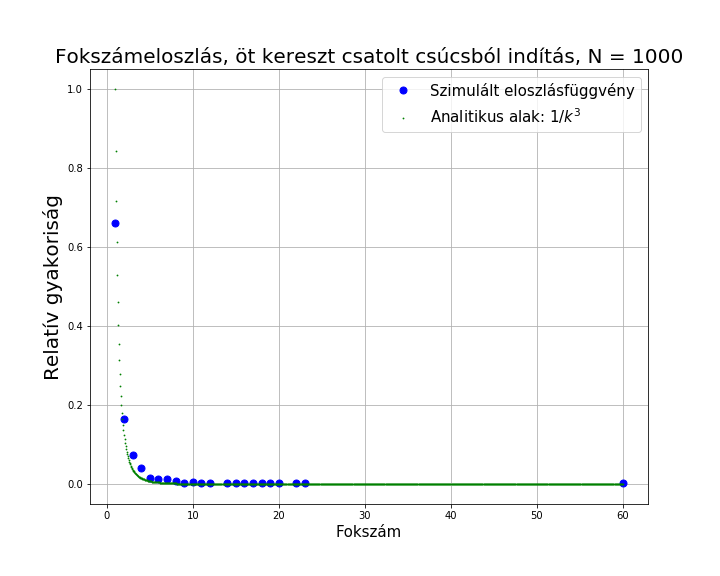
\includegraphics[width=1\textwidth]{harmadik1000.png}
	\end{center}
\end{figure}
\clearpage
\begin{figure}[c!]
	\begin{center}
		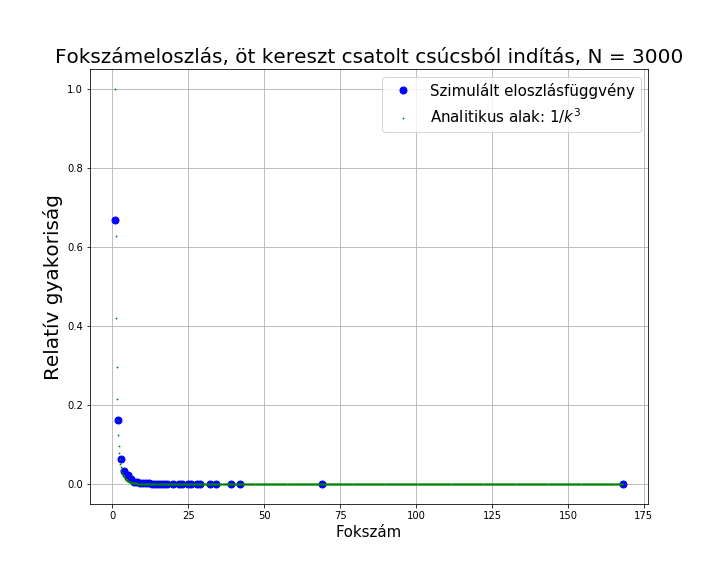
\includegraphics[width=1\textwidth]{harmadik.png}
	\end{center}
\end{figure}
\clearpage

\begin{figure}[ch!]
	\begin{center}
		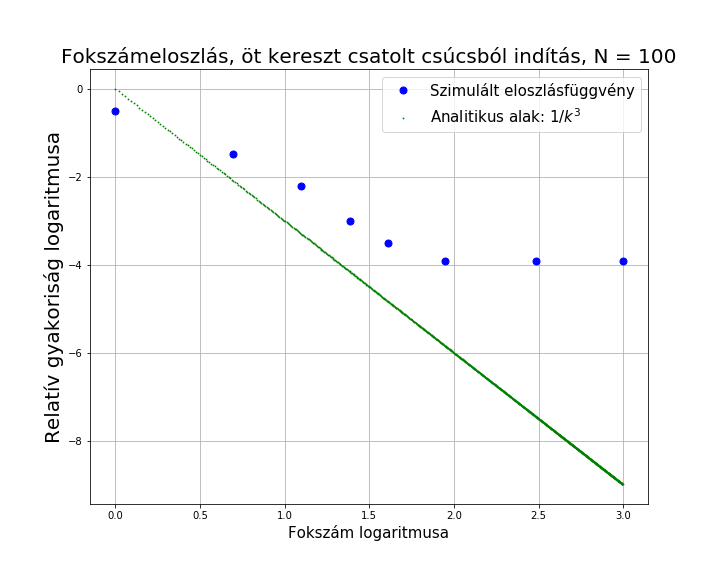
\includegraphics[width=1\textwidth]{harmadik100log.png}
	\end{center}
\end{figure}
\clearpage
\begin{figure}[c!]
	\begin{center}
		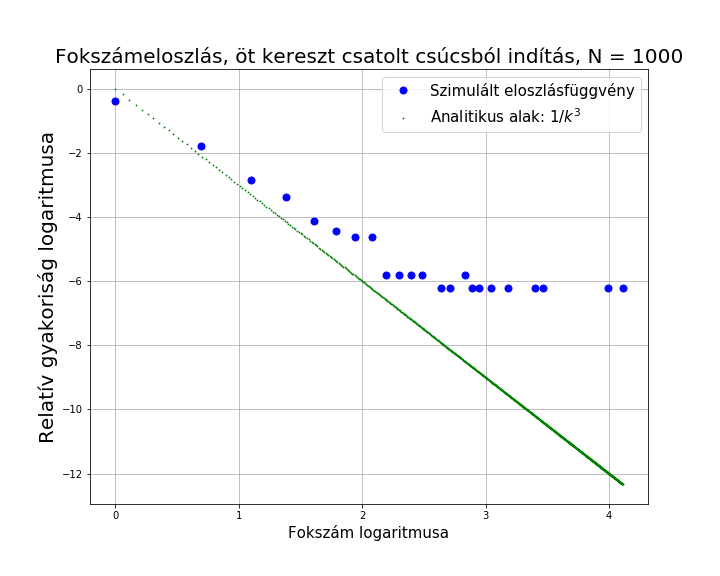
\includegraphics[width=1\textwidth]{harmadik1000log.png}
	\end{center}
\end{figure}
\clearpage
\begin{figure}[c!]
	\begin{center}
		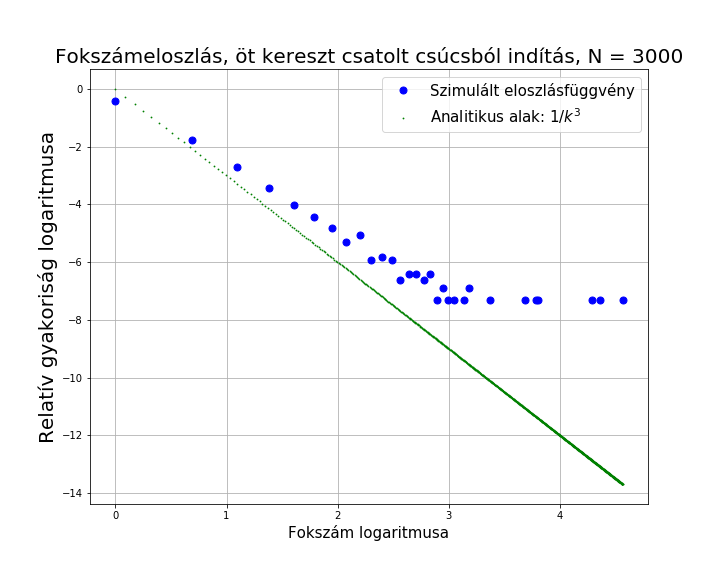
\includegraphics[width=1\textwidth]{harmadik3000log.png}
	\end{center}
\end{figure}
\clearpage



Feladatunk volt megvizsgálni a maximális fokszám átlagának, $\langle k_{max} \rangle$-nak a kezdeti feltételektől való függését.Ebben az esetben úgy jártam el, hogy N = 100, 1000 és 3000 esetére 7-szer lefuttattam a szimulációt mindhárom kezdeti feltételből indítva, lejegyeztem a maximális fokszámú csúcsokat, ezeket kiátlagoltam, és a hibát a következő formulával számoltam:

\begin{center}
	\begin{equation}
	\sigma^2 = \frac{1}{n} \sum_{i = 1}^{n} \left(x_i-\langle x\rangle\right)^2, \rightarrowtail \sigma = \sqrt{\sigma^2}
 	\end{equation}
\end{center}

A mérési adatokat az alábbi táblázatok tartalmazzák. Ezek után kiábrázoltam a kapott $\langle k_{maxi}\rangle$ átlagértékeket hibával együtt, ezt láthatjuk a \ref{Ka} ábrán, amiről leolvashatjuk, hogy mindhárom kezdeti konfiguráció hibahatáron belül közel egyező megoldást ad, illetve mindhárom esetén ahogy várhattuk, N növelésével $\langle k_{maxi}\rangle$ növekvő tendenciát mutat.

\begin{figure}[ht!]
	\begin{center}
		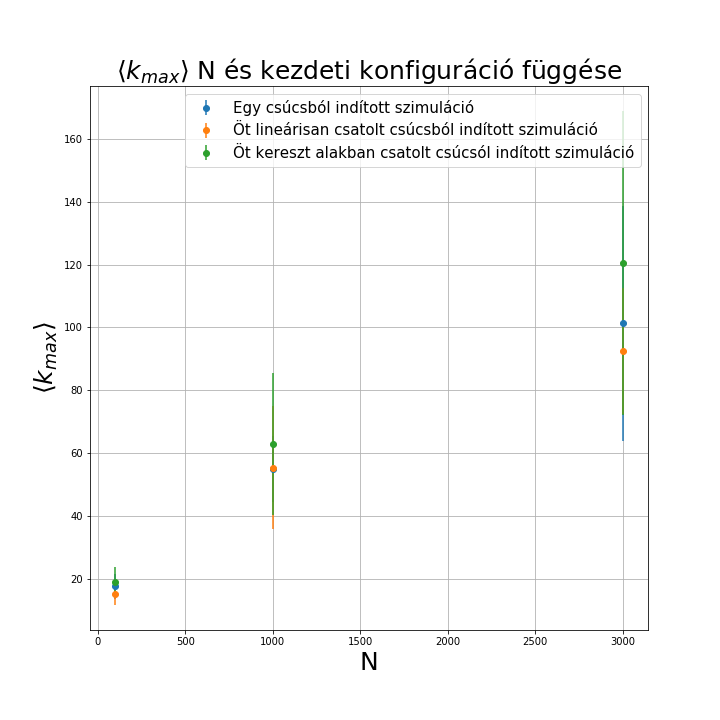
\includegraphics[width=0.8\textwidth]{kmax.png}
	\end{center}
	\caption{$\langle k_{max} \rangle$ N és kezdeti konfiguráció függése.}
	\label{Ka}
\end{figure}

\clearpage

\begin{table}[ht!]
	\captionsetup{justification=centering}
	\begin{center}
		\begin{tabular}{||c|c||}
			\hline
			N & $\langle k_{max} \rangle$ maximális fokszám \\  \hline
			100 & 17 \\	\hline
			100 &15 \\	\hline
			100 & 22\\	\hline
			100 & 20\\	\hline
			100 & 23\\	\hline
			100 & 12\\	\hline
			100 & 14 \\	\hline
			Átlag hibával & 17.57 $\pm$ 3.9\\  \hline
		\end{tabular}
		\caption{$\langle k_{max} \rangle$ maximális fokszámok, s azok átlaga hibával, N = 100 esetre, egy csúcsból indított
			szimuláció esetében.}
	\end{center}
\end{table}

\begin{table}[ht!]
	\captionsetup{justification=centering}
	\begin{center}
		\begin{tabular}{||c|c||}
			\hline
			N & $\langle k_{max} \rangle$ maximális fokszám \\  \hline
			1000 & 57 \\	\hline
			1000 &66 \\	\hline
			1000 &36\\	\hline
			1000 & 58\\	\hline
			1000 & 65\\	\hline
			1000 & 60\\	\hline
			1000 & 43 \\	\hline
			Átlag hibával & 55 $\pm$ 10.4\\  \hline
		\end{tabular}
		\caption{$\langle k_{max} \rangle$ maximális fokszámok, s azok átlaga hibával, N = 1000 esetre, egy csúcsból indított
			szimuláció esetében.}
	\end{center}
\end{table}




\begin{table}[ht!]
	\captionsetup{justification=centering}
	\begin{center}
		\begin{tabular}{||c|c||}
			\hline
			N & $\langle k_{max} \rangle$ maximális fokszám \\  \hline
			3000 & 67 \\	\hline
			3000 &88 \\	\hline
			3000 & 174\\	\hline
			3000 & 116\\	\hline
			3000 & 74\\	\hline
			3000 & 63\\	\hline
			3000 & 127 \\	\hline
			Átlag hibával & 17.57 $\pm$ 3.9\\  \hline
		\end{tabular}
		\caption{$\langle k_{max} \rangle$ maximális fokszámok, s azok átlaga hibával, N = 3000 esetre, egy csúcsból indított
			szimuláció esetében.}
	\end{center}
\end{table}






\begin{table}[ht!]
	\captionsetup{justification=centering}
	\begin{center}
		\begin{tabular}{||c|c||}
			\hline
			N & $\langle k_{max} \rangle$ maximális fokszám \\  \hline
			100 & 23 \\	\hline
			100 &13 \\	\hline
			100 & 17\\	\hline
			100 & 16\\	\hline
			100 & 14\\	\hline
			100 & 13\\	\hline
			100 & 11 \\	\hline
			Átlag hibával & 15.28 $\pm$ 3.7\\  \hline
		\end{tabular}
		\caption{$\langle k_{max} \rangle$ maximális fokszámok, s azok átlaga hibával, N = 100 esetre,öt lineárisan csatolt
			csúcsból indított szimuláció esetében.}
	\end{center}
\end{table}

\begin{table}[ht!]
	\captionsetup{justification=centering}
	\begin{center}
		\begin{tabular}{||c|c||}
			\hline
			N & $\langle k_{max} \rangle$ maximális fokszám \\  \hline
			1000 & 96 \\	\hline
			1000 &46 \\	\hline
			1000 &63\\	\hline
			1000 & 41\\	\hline
			1000 & 46\\	\hline
			1000 & 33\\	\hline
			1000 & 63 \\	\hline
			Átlag hibával & 55.42 $\pm$ 19.5\\  \hline
		\end{tabular}
		\caption{$\langle k_{max} \rangle$ maximális fokszámok, s azok átlaga hibával, N = 1000 esetre, öt lineárisan csatolt
			csúcsból indított szimuláció esetében.}
	\end{center}
\end{table}




\begin{table}[ht!]
	\captionsetup{justification=centering}
	\begin{center}
		\begin{tabular}{||c|c||}
			\hline
			N & $\langle k_{max} \rangle$ maximális fokszám \\  \hline
			3000 & 65 \\	\hline
			3000 &95 \\	\hline
			3000 & 92\\	\hline
			3000 & 125\\	\hline
			3000 & 81\\	\hline
			3000 & 89\\	\hline
			3000 & 109 \\	\hline
			Átlag hibával & 92.42 $\pm$ 20\\  \hline
		\end{tabular}
		\caption{$\langle k_{max} \rangle$ maximális fokszámok, s azok átlaga hibával, N = 3000 esetre, öt lineárisan csatolt
			csúcsból indított szimuláció esetében.}
	\end{center}
\end{table}





\begin{table}[ht!]
	\captionsetup{justification=centering}
	\begin{center}
		\begin{tabular}{||c|c||}
			\hline
			N & $\langle k_{max} \rangle$ maximális fokszám \\  \hline
			100 & 18 \\	\hline
			100 &22  \\	\hline
			100 & 21\\	\hline
			100 & 13\\	\hline
			100 & 13\\	\hline
			100 & 28\\	\hline
			100 & 16 \\	\hline
			Átlag hibával & 19 $\pm$ 4.9\\  \hline
		\end{tabular}
		\caption{$\langle k_{max} \rangle$ maximális fokszámok, s azok átlaga hibával, N = 100 esetre,öt kereszt alakban
			csatolt csúcsból indított szimuláció esetében.}
	\end{center}
\end{table}

\begin{table}[ht!]
	\captionsetup{justification=centering}
	\begin{center}
		\begin{tabular}{||c|c||}
			\hline
			N & $\langle k_{max} \rangle$ maximális fokszám \\  \hline
			1000 & 36 \\	\hline
			1000 &76 \\	\hline
			1000 &38\\	\hline
			1000 & 55\\	\hline
			1000 & 50\\	\hline
			1000 & 86\\	\hline
			1000 & 99 \\	\hline
			Átlag hibával & 62.85 $\pm$ 22.6\\  \hline
		\end{tabular}
		\caption{$\langle k_{max} \rangle$ maximális fokszámok, s azok átlaga hibával, N = 1000 esetre, öt kereszt alakban
			csatolt csúcsból indított szimuláció esetében.}
	\end{center}
\end{table}




\begin{table}[ht!]
	\captionsetup{justification=centering}
	\begin{center}
		\begin{tabular}{||c|c||}
			\hline
			N & $\langle k_{max} \rangle$ maximális fokszám \\  \hline
			3000 & 172 \\	\hline
			3000 &91 \\	\hline
			3000 & 63\\	\hline
			3000 & 85\\	\hline
			3000 & 186\\	\hline
			3000 & 79\\	\hline
			3000 & 168 \\	\hline
			Átlag hibával & 120.57 $\pm$ 48.3\\  \hline
		\end{tabular}
		\caption{$\langle k_{max} \rangle$ maximális fokszámok, s azok átlaga hibával, N = 3000 esetre, öt kereszt alakban
			csatolt csúcsból indított szimuláció esetében.}
	\end{center}
\end{table}





\end{document}